\documentclass[TeamE-eindrapport]{subfiles}

% Jasper zijn deeltje

\begin{document}
	
	\section{Optimale metaparameters bepalen via cross-validation}
	
	\subsection{Metaparameters}
	
	We hebben nu dus twee metaparameters: de variantie en de bias, die bepalen foe flexibel onze grafiek is en hoe dicht ze bij de punten wil aansluiten.	
	
	Met deze metaparameters kunnen de verwachte validatie MSE schrijven in functie van de variantie van de voorspelde waarde van \(x_{0}\), de bias van de voorspelde waarde van \(x_{0}\), en de variantie van de foutterm \(\epsilon\). In \textit{An Introduction to Statistical Learning} \cite{james2023introduction} vinden we de formule \[E(y_{0} - \hat{f}(x_{0}))^{2} = Var(\hat{f}(x_{0}) + [Bias(\hat{f}(x_{0})]^{2} + Var(\epsilon)\] hiervoor terug.
	
	\subsection{Cross-validation}
	
	We proberen nu om de best passende metaparameters te kiezen zodat ons model een zo goed mogelijke voorspelling kan doen. Om deze parameters te kunnen bepalen gebruiken we cross-validation, hierbij delen we onze dataset op in een trainingsdata en een validatiedata. Onze trainingsdata wordt gebruikt om ons model op te stellen en de validatie data wordt hierna op ons model toegepast om de optimate metaparameters te vinden. 
	
	Het is belangrijk dat de validatiedata niet gebruikt wordt om ons model te trainen, we proberen namelijk met onze validatiedata ervoor te zorgen dat ons model algemeen genoeg is en niet enkel geschikt is om voorspellingen te doen op onze trainingsdata. 
	
	\begin{figure}[h!]
		\centering
		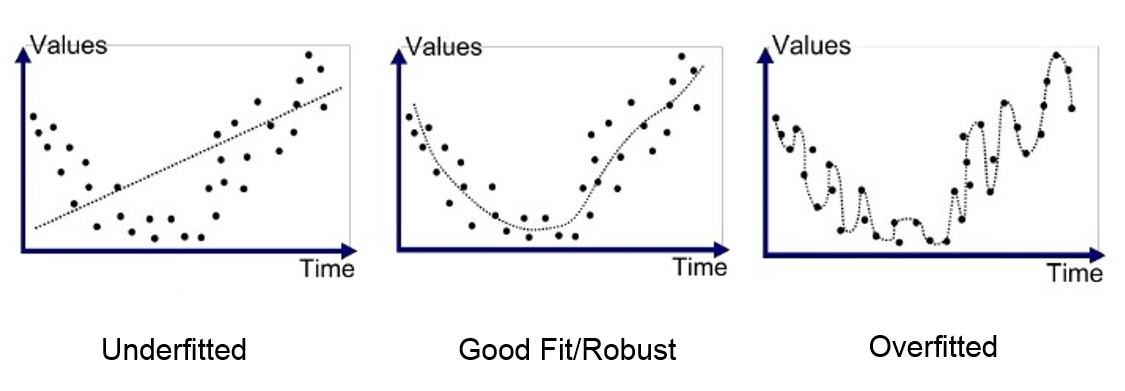
\includegraphics[width=.8\textwidth]{fitting}
		\caption{Illustratie van een underfitting, goeie fit en overfitting. Het eerste  model is duidelijk geen goed model omdat het niet aansluit bij de datapunten. het laatste model zal bij deze dataset een zeer goed model zijn, maar ook enkel voor dit model. Het is niet algemeen genoeg om op nieuwe data toe te passen. We proberen dus het middelste model te vinden die goed bij de punten aansluit maar niet te flexibel is.\cite{Bhande_2018}}
		\label{fig:fitting}
	\end{figure}
	
	Als een model te veel aangepast is aan de trainingsdata noemen we dit overfitting (rechts op figuur \ref{fig:fitting}), het model is dan te flexibel en probeert het model te dicht bij de trainingsdata te liggen. Het is belangrijk dat ons model algemeen is omdat we het model juist willen gebruiken om voorspellingen te doen op nieuwe data en niet op diezelfde trainingsdata, daarvan weten we namelijk al tot welke klasse ze behoren. Als ons model niet dicht genoeg bij de trainingsdata ligt noemen we dit underfitting (links op figuur \ref{fig:fitting}), het model is dan niet flexibel genoeg en er zal ook geen goeie voorspelling gemaakt worden op de validatiedata. We proberen dus de optimale metaparameters te bepalen (midden op figuur \ref{fig:fitting}).
	
\end{document}